% для компиляции в lualatex!!
%\documentclass[12pt, a4paper]{article}
\documentclass[12pt, a4paper]{disser}
\usepackage[english,russian]{babel}
\usepackage[warn]{mathtext}
%\usepackage[T2A]{fontenc}
%\usepackage[utf8]{inputenc}

\usepackage{xecyr} % Продукт Вашего покорного слуги ;)

%\setmainfont{DejaVu Serif}
\setmainfont{Liberation Serif}

\usepackage{color}
\usepackage{amssymb,amsmath}
\usepackage{graphicx}
\usepackage{multicol}

\textheight=24cm           % высота текста
\textwidth=16cm            % ширина текста
\oddsidemargin=0pt         % отступ от левого края
\topmargin=-1.5cm          % отступ от верхнего края
\parindent=24pt            % абзацный отступ
\parskip=0pt               % интервал между абзацами
\tolerance=2000            % терпимость к "жидким" строкам
\flushbottom               % выравнивание высоты страниц
%\def\baselinestretch{1.5} % печать с большим интервалом

%\title{}
%\author{\copyright~~С.А.~Назарова \thanks{e-mail:~sophia.nazarova@gmail.com}}
%\date{}


\begin{document}

	\begin{figure}[ht]
	
	\begin{minipage}[b]{.46\linewidth}
	%Фигурка в первом ряду слева размер отведенный под весь этот объект \textendash 0.46 от ширины строки
	%Параметр [b] означает, что выравнивание этих министраниц будет по нижнему краю
	\begin{center}
		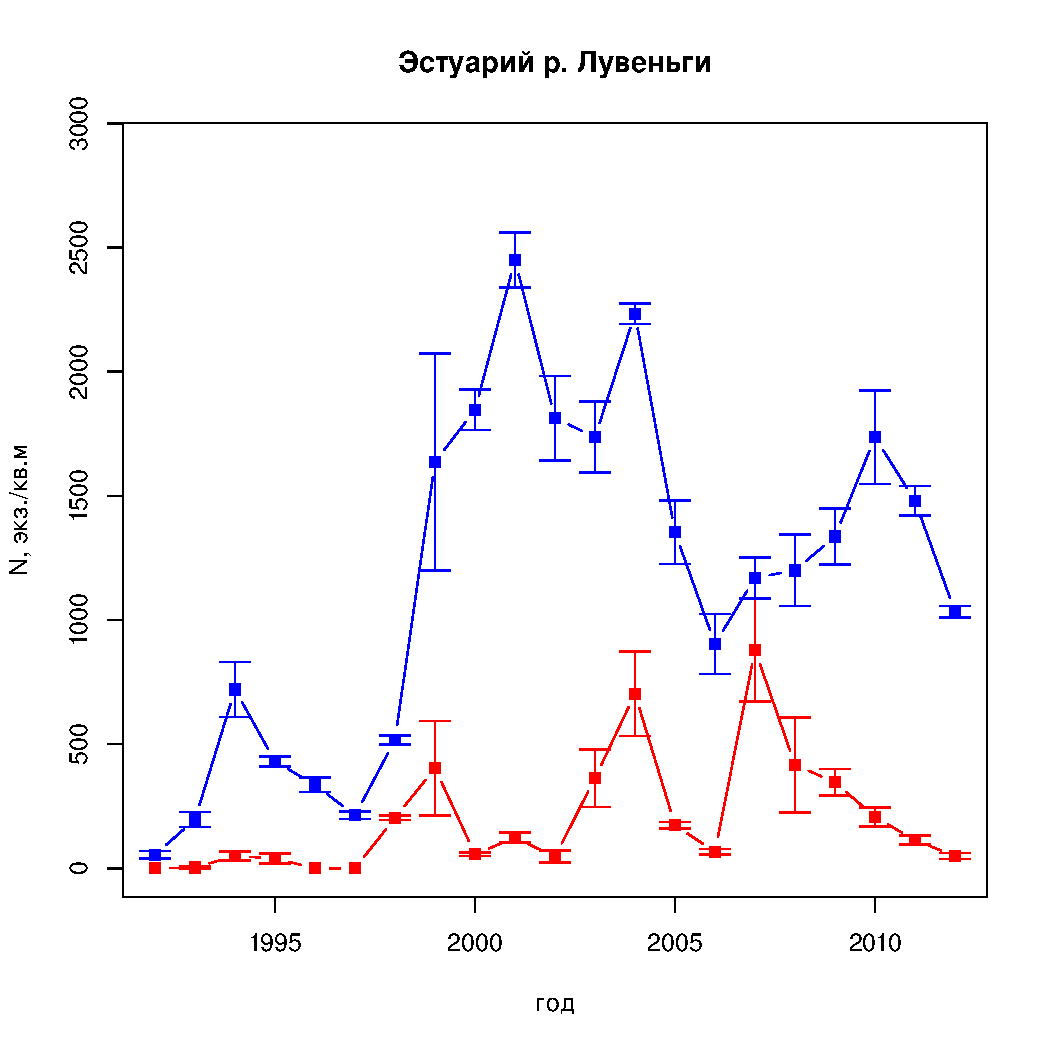
\includegraphics[width=65mm]{../White_Sea/Estuatiy_Luvenga/Estuary_N1_Nold.pdf}

	\end{center}
	\end{minipage}
	%
	\hfil %Это пружинка отодвигающая рисунки друг от друга
	%
	\begin{minipage}[b]{.46\linewidth}
	\begin{center}
		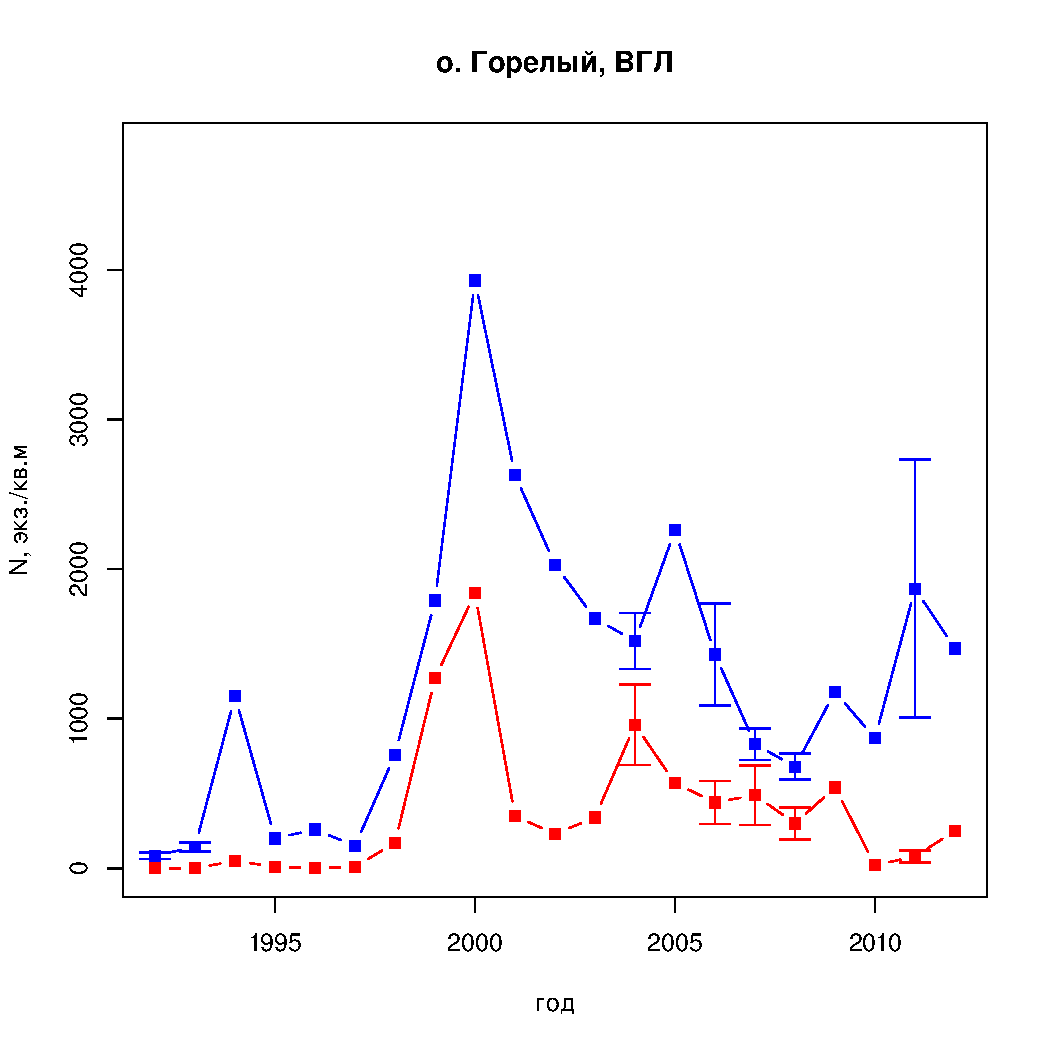
\includegraphics[width=65mm]{../White_Sea/Luvenga_Goreliy/Goreliy_high_N1_Nold.pdf}
	\end{center}
	\end{minipage}

%\smallskip


	\begin{minipage}[b]{.46\linewidth}
%Фигурка в первом ряду слева размер отведенный под весь этот объект \textendash 0.46 от ширины строки
%Параметр [b] означает, что выравнивание этих министраниц будет по нижнему краю
	\begin{center}
		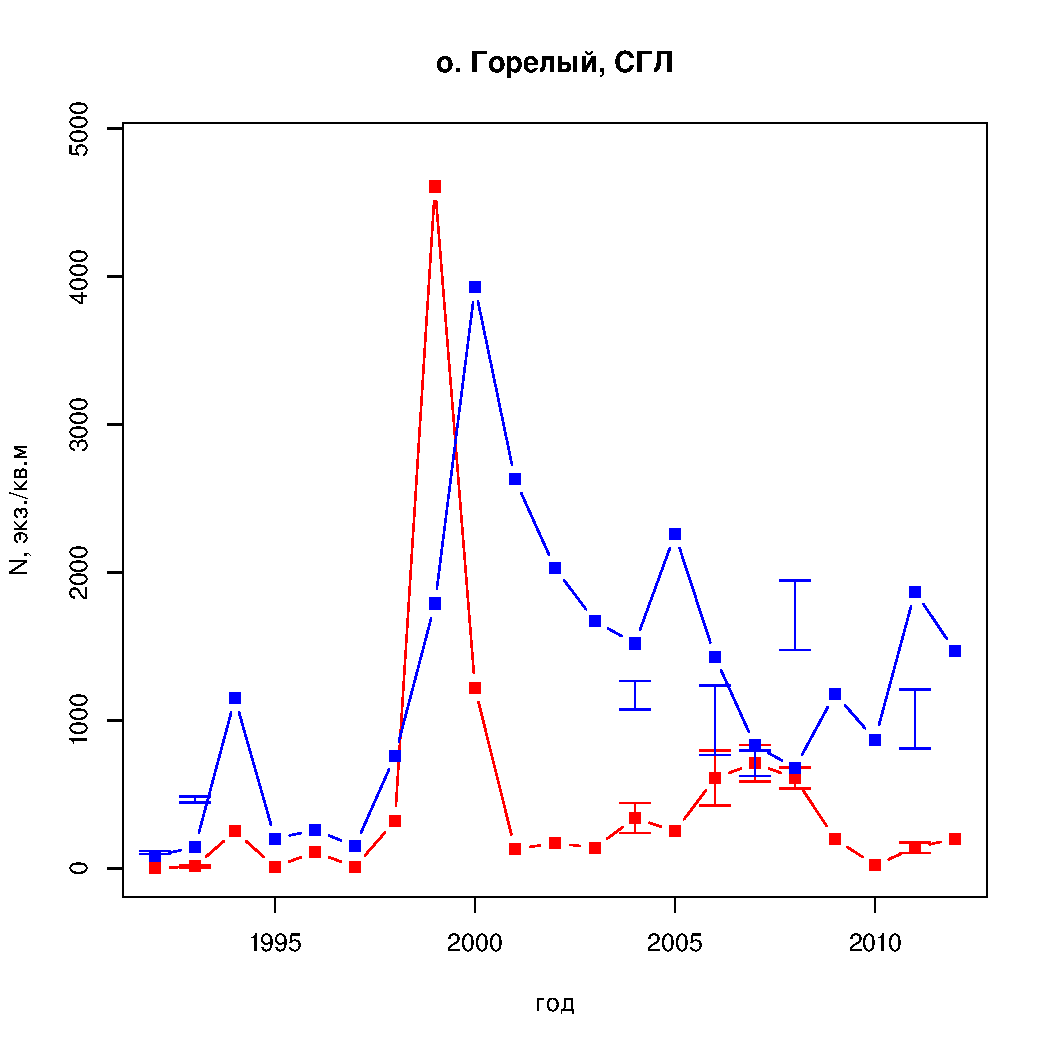
\includegraphics[width=65mm]{../White_Sea/Luvenga_Goreliy/Goreliy_middle_N1_Nold.pdf}
	\end{center}
	\end{minipage}
%
	\hfil %Это пружинка отодвигающая рисунки друг от друга
%
	\begin{minipage}[b]{.46\linewidth}
%Следующий рисунок - первый ряд справа %DUNGEON S_4 \ AB
	\begin{center}	
		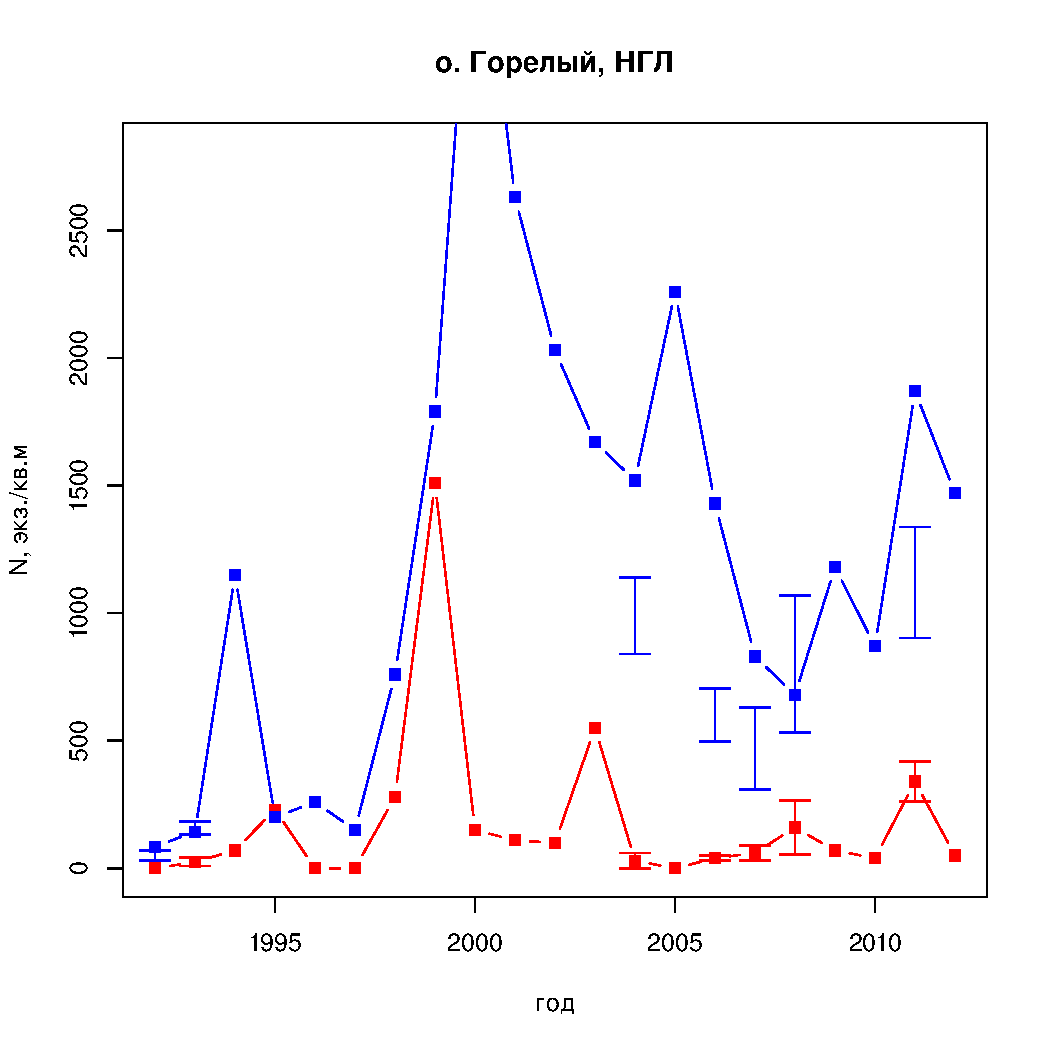
\includegraphics[width=65mm]{../White_Sea/Luvenga_Goreliy/Goreliy_midlow_N1_Nold.pdf}
	\end{center}
	\end{minipage}

%\smallskip

	\begin{minipage}[b]{.46\linewidth}
%Фигурка в первом ряду слева размер отведенный под весь этот объект \textendash 0.46 от ширины строки
%Параметр [b] означает, что выравнивание этих министраниц будет по нижнему краю
	\begin{center}
		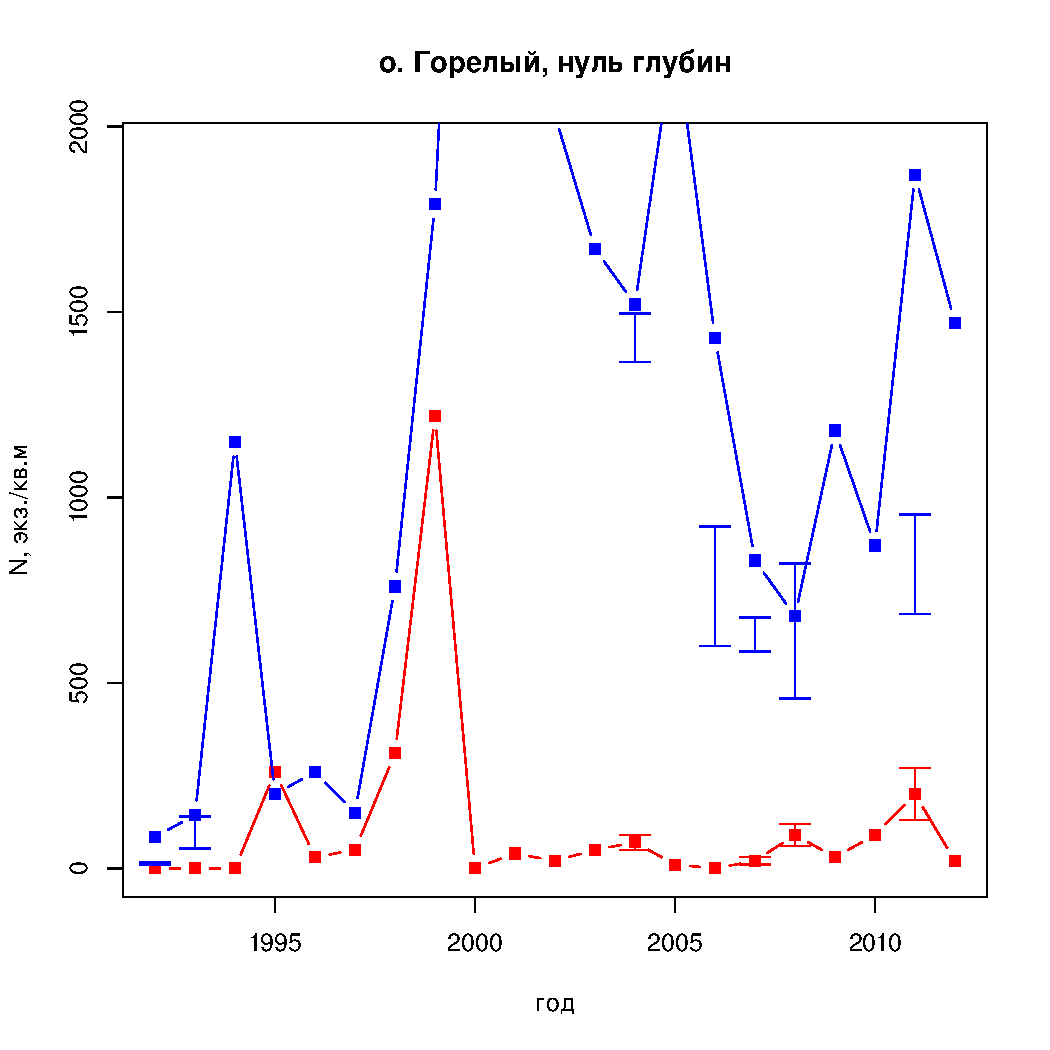
\includegraphics[width=65mm]{../White_Sea/Luvenga_Goreliy/Goreliy_low_N1_Nold.pdf}
	\end{center}
	\end{minipage}
%
	\hfil %Это пружинка отодвигающая рисунки друг от друга
%
	\begin{minipage}[b]{.46\linewidth}
%Следующий рисунок - первый ряд справа %DUNGEON S_4 \ AB
	\begin{center}
		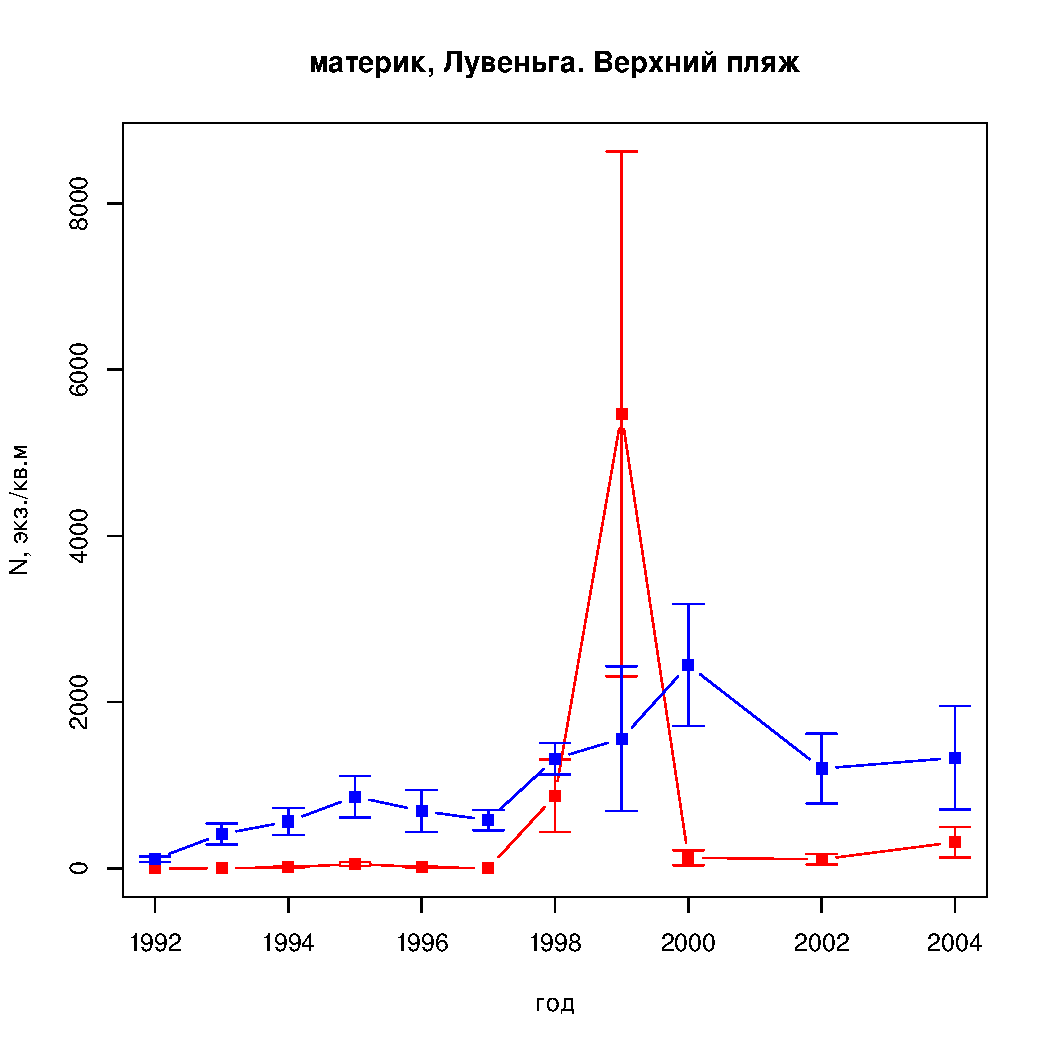
\includegraphics[width=65mm]{../White_Sea/Luvenga_II_razrez/2razrez_high_beatch_N1_Nold.pdf}
	\end{center}
	\end{minipage}

%\smallskip
	\caption{Соотношение динамики годовалых {\it Macoma balthica} (красная линия) и и старших особей (синяя линия) в Кандалакшском заливе}
	\label{ris:N1_Nold_Kandalaksha}
	\end{figure}




	\begin{figure}[ht]
	
	\begin{minipage}[b]{.46\linewidth}
	%Фигурка в первом ряду слева размер отведенный под весь этот объект \textendash 0.46 от ширины строки
	%Параметр [b] означает, что выравнивание этих министраниц будет по нижнему краю
	\begin{center}
		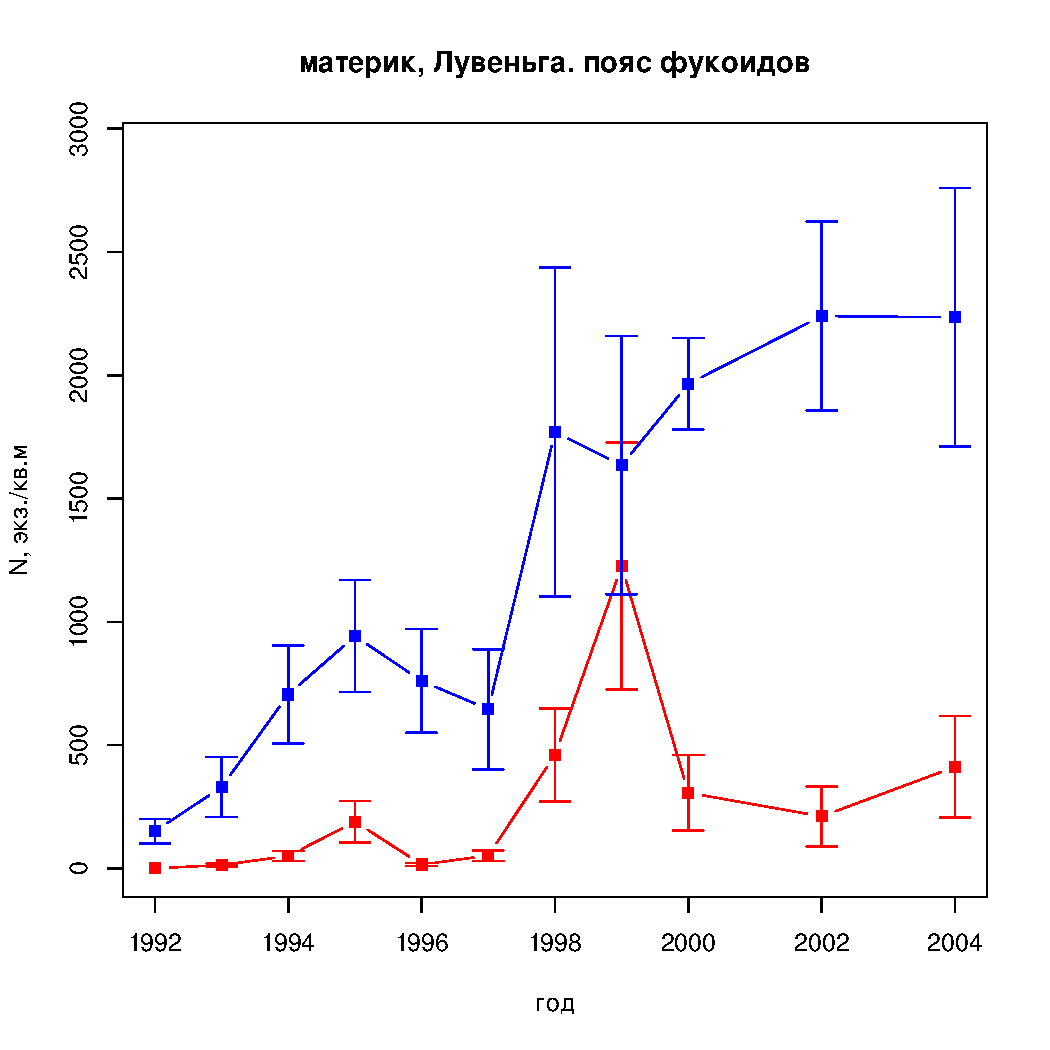
\includegraphics[width=65mm]{../White_Sea/Luvenga_II_razrez/2razrez_fucus_zone_N1_Nold.pdf}
	\end{center}
	\end{minipage}
	%
	\hfil %Это пружинка отодвигающая рисунки друг от друга
	%
	\begin{minipage}[b]{.46\linewidth}
%Следующий рисунок - первый ряд справа %DUNGEON S_4 \ AB
	\begin{center}
		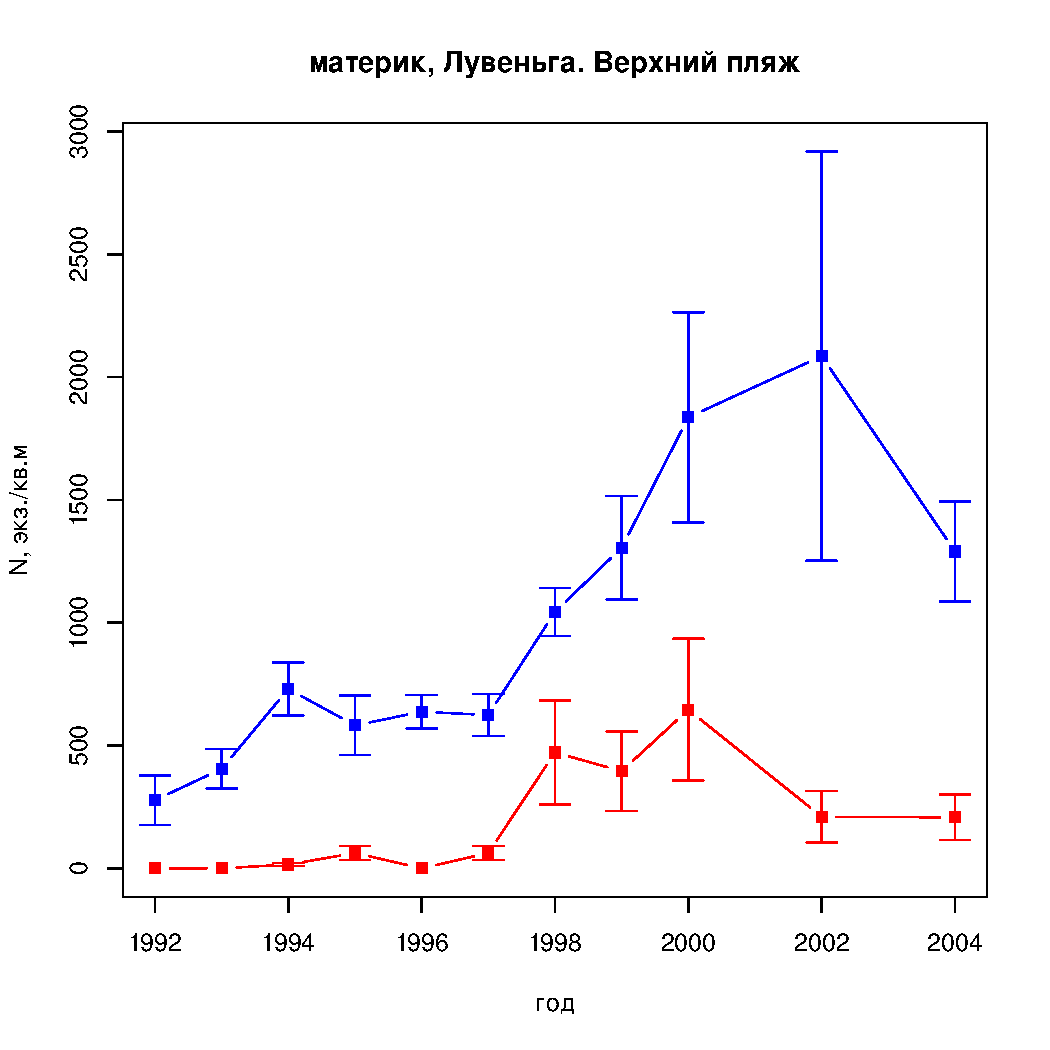
\includegraphics[width=65mm]{../White_Sea/Luvenga_II_razrez/2razrez_zostera_zone_N1_Nold.pdf}
	\end{center}
	\end{minipage}

%\smallskip


	\begin{minipage}[b]{.46\linewidth}
%Фигурка в первом ряду слева размер отведенный под весь этот объект \textendash 0.46 от ширины строки
%Параметр [b] означает, что выравнивание этих министраниц будет по нижнему краю
	\begin{center}
		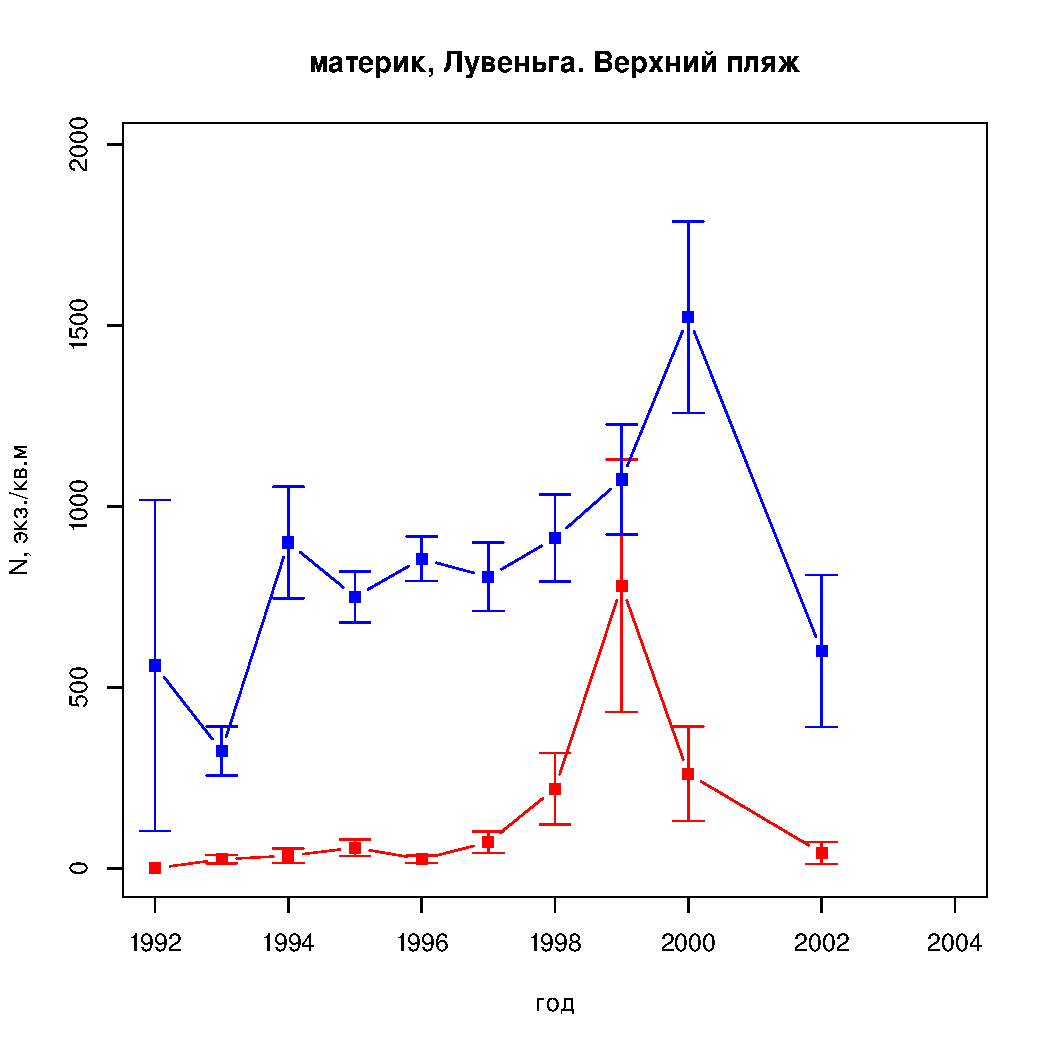
\includegraphics[width=65mm]{../White_Sea/Luvenga_II_razrez/2razrez_low_beatch_N1_Nold.pdf}
	\end{center}
	\end{minipage}
%
	\hfil %Это пружинка отодвигающая рисунки друг от друга
%
	\begin{minipage}[b]{.46\linewidth}
%Следующий рисунок - первый ряд справа %DUNGEON S_4 \ AB
	\begin{center}	
		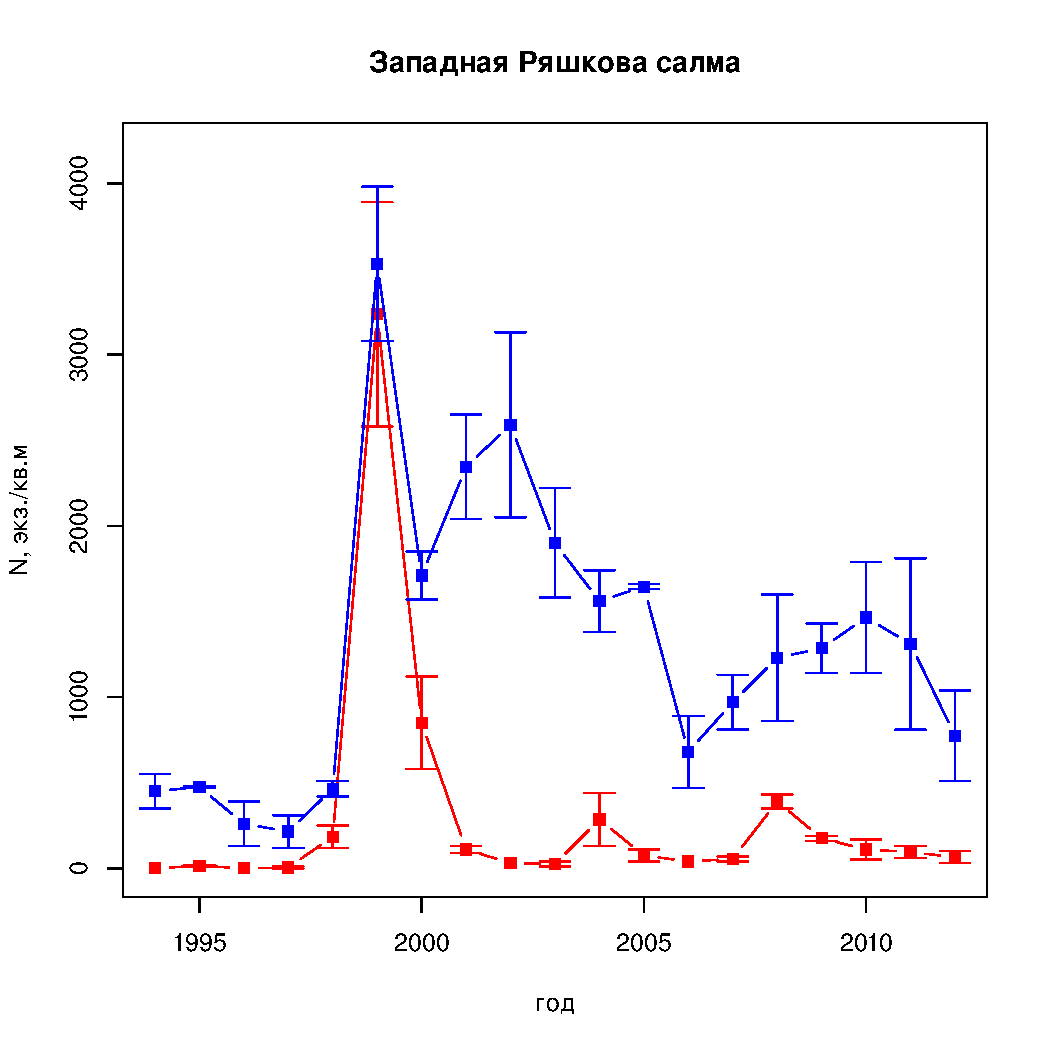
\includegraphics[width=65mm]{../White_Sea/Ryashkov_ZRS/ZRS_N1_Nold.pdf}
	\end{center}
	\end{minipage}

%\smallskip

	\begin{minipage}[b]{.46\linewidth}
%Фигурка в первом ряду слева размер отведенный под весь этот объект \textendash 0.46 от ширины строки
%Параметр [b] означает, что выравнивание этих министраниц будет по нижнему краю
	\begin{center}
		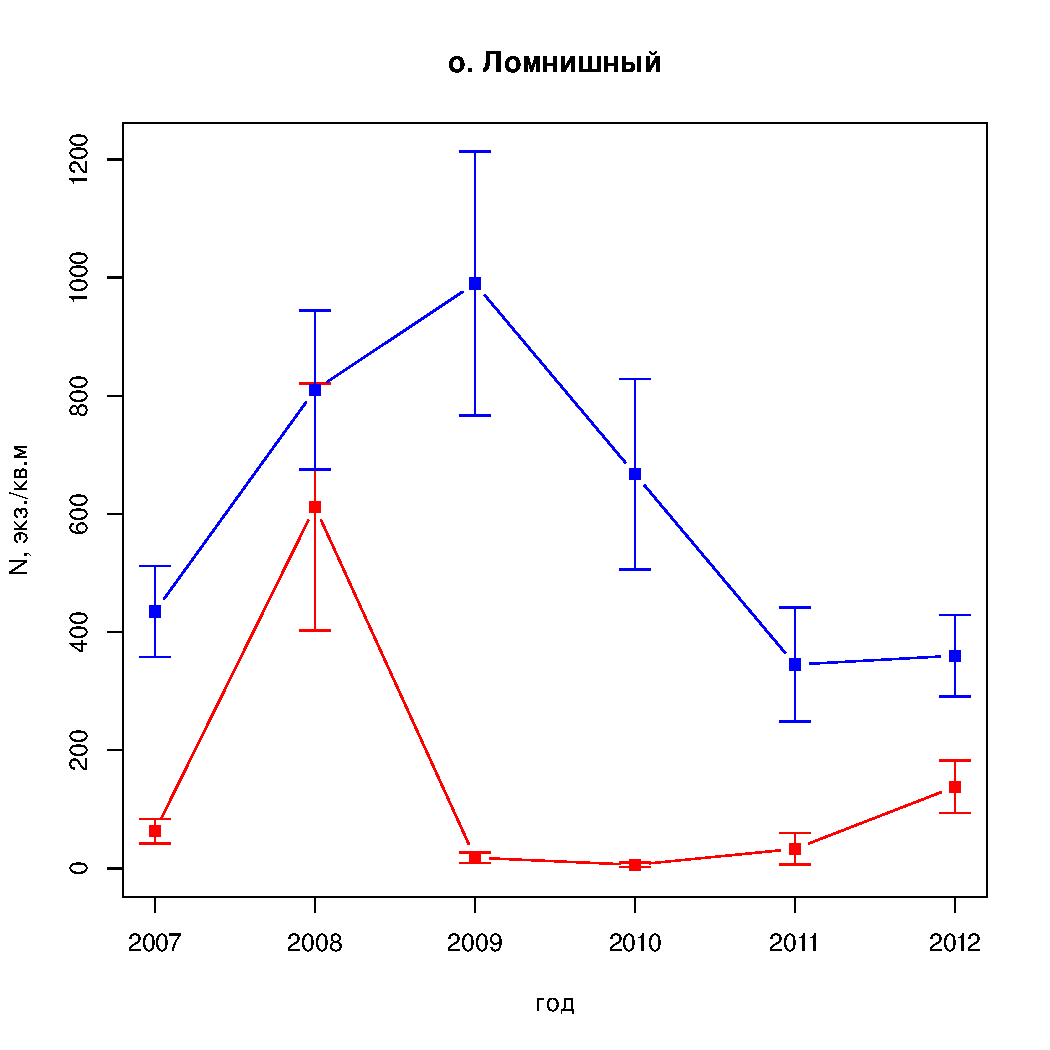
\includegraphics[width=65mm]{../White_Sea/Lomnishniy/Lomnishniy_N1_Nold.pdf}
	\end{center}
	\end{minipage}
%
	\hfil %Это пружинка отодвигающая рисунки друг от друга
%
	\begin{minipage}[b]{.46\linewidth}
%Следующий рисунок - первый ряд справа %DUNGEON S_4 \ AB
	\begin{center}
	{\tiny Южная губа}
	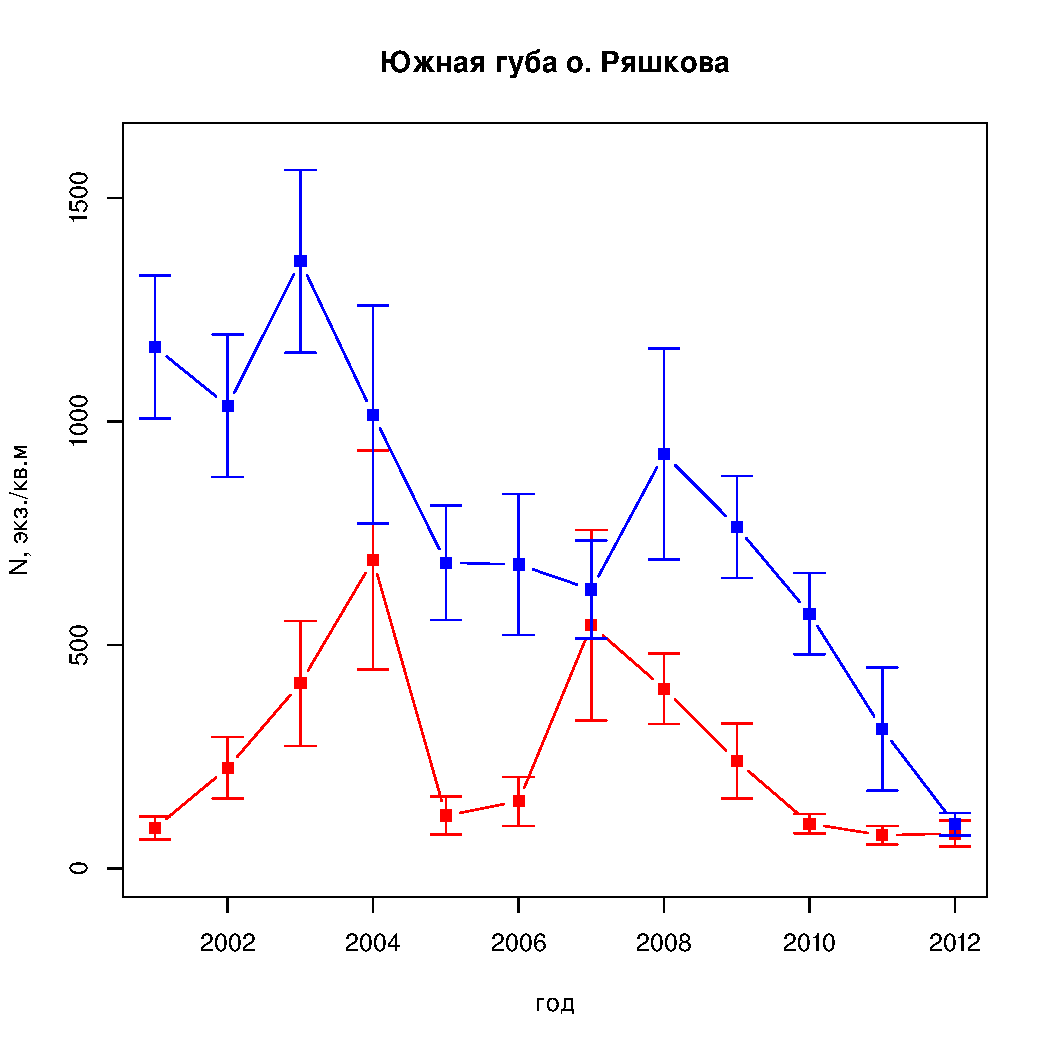
\includegraphics[width=65mm]{../White_Sea/Ryashkov_YuG/YuG_N1_Nold.pdf}
	\end{center}
	\end{minipage}

%\smallskip
%	\caption{Динамика плотности поселений {\it Macoma balthica} в вершине Кандалакшского залива}
%	\label{ris:dynamic_Kandalaksha_all}
\begin{center}
Рисунок \ref{ris:N1_Nold_Kandalaksha}, продолжение. Соотношение динамики годовалых {\it Macoma balthica} (красная линия) и старших особей (синяя линия) в Кандалакшском заливе
\end{center}
	\end{figure}

\end{document}
